\documentclass[
  xcolor={svgnames},
  hyperref={colorlinks,citecolor=DeepPink4,linkcolor=DarkRed,urlcolor=DarkBlue}
  ]{beamer}
\usepackage{amsmath}
\usepackage{amssymb}
\usepackage{amsfonts}
\usepackage[utf8]{inputenc}
\usepackage{graphicx}
\usepackage{hyperref}
\usepackage{xcolor}
\usepackage{wasysym}
\usepackage{listings}
\usepackage{tikz}
\usepackage[normalem]{ulem}
\usepackage{textcomp}
\usepackage{verbatim}
\usepackage[T1]{fontenc}
\usepackage{lmodern}
\usepackage[framemethod=tikz]{mdframed}

\usetikzlibrary{shapes.callouts,shadows, calc}

\tikzset{note/.style={rectangle callout, rounded corners,fill=gray!20,drop shadow,font=\footnotesize}}    
\newcommand{\tikzmark}[1]{\tikz[overlay,remember picture] \node (#1) {};}    

\newcounter{image}
\setcounter{image}{1}

\makeatletter
\newenvironment{btHighlight}[1][]
{\begingroup\tikzset{bt@Highlight@par/.style={#1}}\begin{lrbox}{\@tempboxa}}
{\end{lrbox}\bt@HL@box[bt@Highlight@par]{\@tempboxa}\endgroup}

\newcommand\btHL[1][]{%
  \begin{btHighlight}[#1]\bgroup\aftergroup\bt@HL@endenv%
}
\def\bt@HL@endenv{%
  \end{btHighlight}%   
  \egroup
}
\newcommand{\bt@HL@box}[2][]{%
  \tikz[#1]{%
    \pgfpathrectangle{\pgfpoint{0pt}{0pt}}{\pgfpoint{\wd #2}{\ht #2}}%
    \pgfusepath{use as bounding box}%
    \node[anchor=base west,rounded corners, fill=green!30,outer sep=0pt,inner xsep=0.2em, inner ysep=0.1em,  #1](a\theimage){\usebox{#2}};
  }%
 \stepcounter{image}
}
\makeatother

\usetheme{Warsaw}
\usecolortheme{lily}
\setbeamercovered{transparent}
\setbeamertemplate{headline}{
  \begin{beamercolorbox}{section in head/foot}
    \vskip2pt\insertnavigation{\paperwidth}\vskip2pt
  \end{beamercolorbox}
}

\setbeamertemplate{footline}{
}

\author{
  {\tiny Tony Morris\\}
}

\xdefinecolor{darkgreen}{rgb}{0,0.35,0}
\lstset{
  tabsize=2,
  basicstyle=\ttfamily,
  moredelim=**[is][\btHL]{`}{`}
}
\lstdefinelanguage{java}{
  morekeywords={abstract,assert,boolean,break%
    byte,case,catch,char,class,const,continue%
    default,do,double,else,enum,extends,false%
    final,finally,float,for,goto,if,implements%
    import,instanceof,int,interface,long,native%
    new,null,package,private,protected,public%
    return,short,static,strictfp,super,switch%
    synchronized,this,throw,throws,transient%
    true,try,void,volatile,while},
  otherkeywords={=,=>,<-,<\%,<:,>:,\#,@},
  sensitive=true,
  morecomment=[l]{//},
  morecomment=[n]{/*}{*/},
  morestring=[b]",
  morestring=[b]',
  morestring=[b]"""
}
\lstdefinelanguage{csharp}
{
  sensitive=true,
  morekeywords=[1]{
  abstract, as, base, break, case,
  catch, checked, class, const, continue,
  default, delegate, do, else, enum,
  event, explicit, extern, false,
  finally, fixed, for, foreach, goto, if,
  implicit, in, interface, internal, is,
  lock, namespace, new, null, operator,
  out, override, params, private,
  protected, public, readonly, ref,
  return, sealed, sizeof, stackalloc,
  static, struct, switch, this, throw,
  true, try, typeof, unchecked, unsafe,
  using, virtual, volatile, while, bool,
  byte, char, decimal, double, float,
  int, lock, object, sbyte, short, string,
  uint, ulong, ushort, void},
  morecomment=[l]{//},
  morecomment=[s]{/*}{*/},
  morecomment=[l][keywordstyle4]{\#},
  morestring=[b]",
  morestring=[b]',
}
\lstdefinelanguage{haskell}{
  morekeywords={class,instance,where,do,data,newtype,default,deriving,module},
  otherkeywords={<-},
  sensitive=true,
  morecomment=[l]{--},
  morecomment=[n]{\{-}{-\}}, 
  morestring=[b]",
  morestring=[b]',
  morestring=[b]"""
}
\lstdefinelanguage{python}{
 keywords={catch, def, float, lambda, in, int, null, self, str, switch, typeof},
 keywordstyle=\color{ForestGreen}\bfseries,
 ndkeywords={boolean, throw, import},
 ndkeywords={return, class, if ,elif, endif, while, do, else, True, False , catch, def},
 ndkeywordstyle=\color{red}\bfseries,
 identifierstyle=\color{black},
 sensitive=false,
 comment=[l]{\#},
 morecomment=[s]{/*}{*/},
 commentstyle=\color{purple}\ttfamily,
 stringstyle=\color{red}\ttfamily,
}
\lstdefinelanguage{scala}{
  morekeywords={abstract,case,catch,class,def,%
    do,else,extends,false,final,finally,%
    for,forSome,if,implicit,import,lazy,match,%
    new,null,object,override,package,%
    private,protected,requires,return,sealed,%
    super,this,throw,trait,true,try,%
    type,val,var,while,with,yield},
  otherkeywords={=,=>,<-,<\%,<:,>:,\#,@},
  sensitive=true,
  morecomment=[l]{//},
  morecomment=[n]{/*}{*/},
  morestring=[b]",
  morestring=[b]',
  morestring=[b]"""
}
\lstdefinestyle{haskell}{
  language=haskell,
  basicstyle=\tiny\ttfamily,
  stringstyle=\color{darkgreen}\ttfamily,
  commentstyle=\color{gray}\ttfamily,
  keywordstyle=\footnotesize\color{blue}\ttfamily,
  tabsize=2,
  moredelim=**[is][\btHL]{`}{`}
}
\lstdefinestyle{java}{
  language=java,
  basicstyle=\footnotesize\ttfamily,
  stringstyle=\color{darkgreen}\ttfamily,
  commentstyle=\color{gray}\ttfamily,
  keywordstyle=\footnotesize\color{blue}\ttfamily,
  tabsize=2,
  moredelim=**[is][\btHL]{`}{`}
}
\lstdefinestyle{python}{
  language=python,
  basicstyle=\footnotesize\ttfamily,
  stringstyle=\color{darkgreen}\ttfamily,
  commentstyle=\color{gray}\ttfamily,
  keywordstyle=\footnotesize\color{blue}\ttfamily,
  tabsize=2,
  moredelim=**[is][\btHL]{`}{`}
}
\lstdefinestyle{csharp}{
  language=csharp,
  basicstyle=\tiny\ttfamily,
  stringstyle=\color{darkgreen}\ttfamily,
  commentstyle=\color{gray}\ttfamily,
  keywordstyle=\tiny\color{blue}\ttfamily,
  tabsize=2,
  moredelim=**[is][\btHL]{`}{`}
}
\lstdefinestyle{scala}{
  language=scala,
  basicstyle=\footnotesize\ttfamily,
  stringstyle=\color{darkgreen}\ttfamily,
  commentstyle=\color{gray}\ttfamily,
  keywordstyle=\footnotesize\color{blue}\ttfamily,
  tabsize=2,
  moredelim=**[is][\btHL]{`}{`}
}
% #866eaa
\definecolor{nicta-purple}{rgb}{0.5234,0.4297,0.6640}

\defbeamertemplate*{title page}{customized}[1][] {
  \centering
  \color{nicta-purple}
  \usebeamerfont{title}\inserttitle\par
  \bigskip
  \usebeamerfont{subtitle}\insertsubtitle\par
  \bigskip
  \bigskip
  \bigskip
  \bigskip
  \usebeamerfont{institute}\insertinstitute\par
  \bigskip
  \usebeamerfont{author}\insertauthor\par
  % \usebeamerfont{date}\insertdate\par
  \usebeamercolor[fg]{titlegraphic}\inserttitlegraphic
}

\logo{
\includegraphics[height=0.8cm]{image/data61-csiro.jpg}}


\setbeamercovered{transparent}

\begin{document}

\newmdenv[tikzsetting={draw=black,fill=white,fill opacity=0.7, line width=4pt},backgroundcolor=none,leftmargin=0,rightmargin=0,innertopmargin=4pt]{Conference}

\newmdenv[tikzsetting={draw=black,fill=white,fill opacity=0.7, line width=4pt},backgroundcolor=none,leftmargin=0,rightmargin=0,innertopmargin=4pt,skipbelow=\baselineskip,%
skipabove=\baselineskip]{TitleBox}

\title{\large Parametricity}
\subtitle{\large Types are Documentation}
\institute[Data61]{Data61, CSIRO}

{
  \usebackgroundtemplate{
\includegraphics[width=1.0\paperwidth]{image/lambda.png}}

  \begin{frame}[plain] 

  \begin{TitleBox}
    \begin{center}
    {\huge \inserttitle}

    \hspace{1em}
    
    {\huge \insertsubtitle}
    \end{center}
  \end{TitleBox}

  \vspace{3em}

  \begin{Conference}
    \begin{center}
    \tiny{CanFP, Canberra, July 2018}

    \hspace{1em}

    {\insertauthor}
    \end{center}
  \end{Conference}

  \end{frame}

}

\begin{frame}
\frametitle{QFPL}
\begin{block}{http://qfpl.io/}
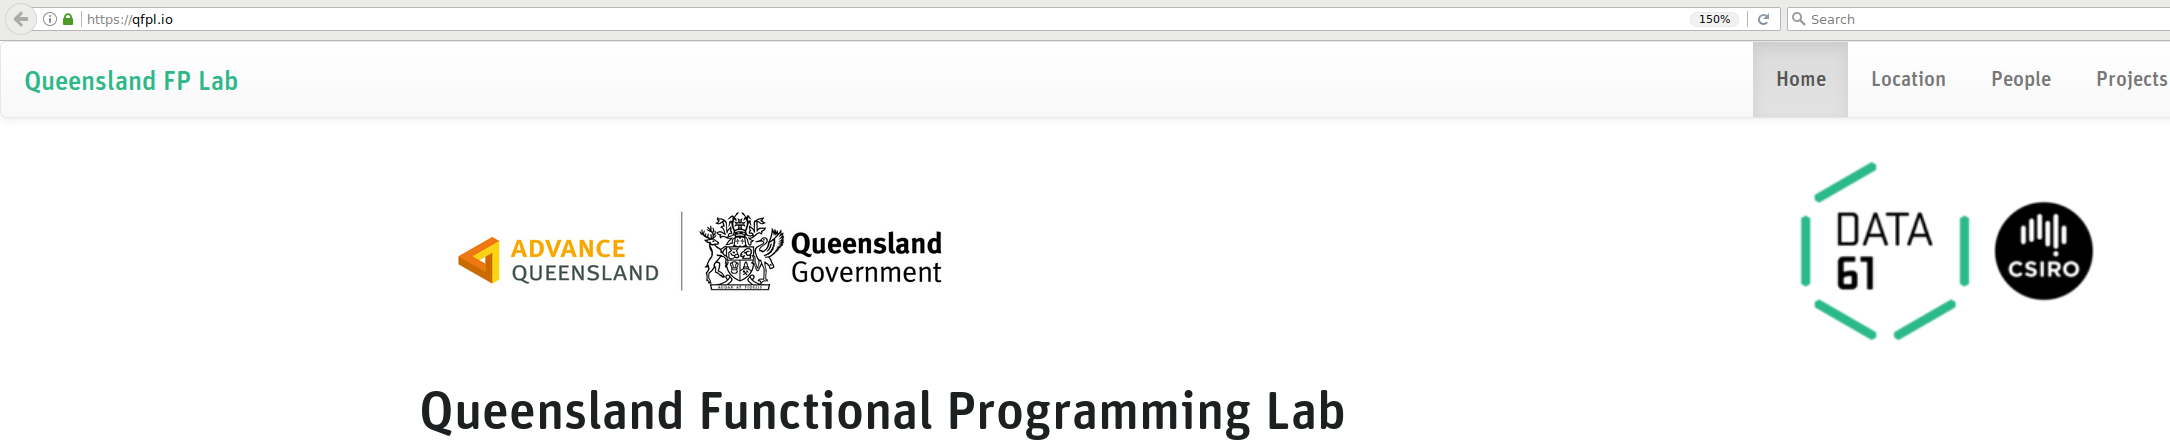
\includegraphics[height=0.24\textheight]{image/qfpl-io.png}
\end{block}
\end{frame}

\begin{frame}
\frametitle{Frequently Asked Questions}
\begin{block}{FAQ}
\begin{itemize}
\item<1-> \textbf{How can I be notified of upcoming FP courses?}
  \begin{itemize}
  \item Subscribe to this mailing list

        \url{http://notify.qfpl.io/}
  \item Sign up to YOW! conference notifications
  \end{itemize}
\item<2-> \textbf{Do you do non-introductory FP courses?}

  Starting in 2018. Sign up to notifications.
\end{itemize}
\end{block}
\end{frame}

\begin{frame}
\begin{center}
Let us remind ourselves.
\end{center}
\begin{center}
What is Functional Programming? What does it \emph{mean}?
\end{center}
\end{frame}

\begin{frame}[fragile]
\begin{block}{Suppose the following program \ldots}
\begin{lstlisting}[style=java]
int wibble(int a, int b) {
  counter = counter + 1;
  return (a + b) * 2;
}

/* arbitrary code */

blobble(wibble(x, y), wibble(x, y));
\end{lstlisting}
\end{block}
\end{frame}

\begin{frame}[fragile]
\begin{block}{and we refactor out these common expressions \ldots}
\begin{lstlisting}[style=java]
int wibble(int a, int b) {
  counter = counter + 1;
  return (a + b) * 2;
}

/* arbitrary code */

blobble(`wibble(x, y)`, `wibble(x, y)`);
\end{lstlisting}
\end{block}
\end{frame}

\begin{frame}[fragile]
\begin{block}{assign the expression to a value}
\begin{lstlisting}[style=java]
int wibble(int a, int b) {
  counter = counter + 1;
  return (a + b) * 2;
}

int r = `wibble(x, y);`

/* arbitrary code */

blobble(`r`, `r`);
\end{lstlisting}
\end{block}
\end{frame}

\begin{frame}[fragile]
\begin{center}
Did the program just change?
\end{center}
\end{frame}

\begin{frame}[fragile]
\begin{block}{Yes, the program changed \ldots}
\begin{lstlisting}[style=java]
int wibble(int a, int b) {
  `counter = counter + 1;`
  return (a + b) * 2;
}

int r = wibble(x, y);

/* arbitrary code */

blobble(r, r);
\end{lstlisting}
\end{block}
\end{frame}

\begin{frame}[fragile]
\begin{block}{Suppose this slightly different program \ldots}
\begin{lstlisting}[style=java]
int pibble(int a, int b) {
  return (a + b) * 2;
}

/* arbitrary code */

globble(pibble(x, y), pibble(x, y));
\end{lstlisting}
\end{block}
\end{frame}

\begin{frame}[fragile]
\begin{block}{and we refactor out these common expressions \ldots}
\begin{lstlisting}[style=java]
int pibble(int a, int b) {
  return (a + b) * 2;
}

/* arbitrary code */

globble(`pibble(x, y)`, `pibble(x, y)`);
\end{lstlisting}
\end{block}
\end{frame}

\begin{frame}[fragile]
\begin{block}{assign the expression to a value}
\begin{lstlisting}[style=java]
int pibble(int a, int b) {
  return (a + b) * 2;
}

int r = `pibble(x, y);`

/* arbitrary code */

globble(`r`, `r`);
\end{lstlisting}
\end{block}
\end{frame}

\begin{frame}
\begin{center}
This time, did the program just change?
\end{center}
\end{frame}

\begin{frame}
\begin{block}{It's the same program}
For given inputs, the same outputs are given, with no observable changes to the program
\end{block}
\end{frame}

\begin{frame}
\begin{block}{Functional Programming is the idea that}
We can \textbf{always replace expressions with a value, without affecting the program behaviour}
\end{block}
\begin{center}
\tiny{This property of expressions is called \emph{referential transparency}.}
\end{center}
\end{frame}
\begin{frame}
\begin{block}{Consequences}
A commitment to Functional Programming has many consequences.
\end{block}
\end{frame}

\begin{frame}
\begin{center}
One of the most important and practical of those is
\end{center}
\begin{center}
\textbf{Parametricity}
\end{center}
\end{frame}

\begin{frame}
\frametitle{What is Parametricity}
\begin{block}{Philip Wadler \cite{wadler1989theorems} tells us:}
\begin{quotation}
Write down the definition of a polymorphic function on a piece of paper. Tell me its type, but be careful not to let me see the function's definition. I will tell you a theorem that the function satisfies.

The purpose of this paper is to explain the trick.
\end{quotation}
\end{block}
\end{frame}

\begin{frame}[fragile]
\frametitle{Types}
\begin{block}{first let's talk about types}
Suppose we encountered the following function definition:
\begin{lstlisting}
int add12(int)
\end{lstlisting}
\end{block}
\begin{itemize}
  \item<1-> by the type alone, there are {$({2^{32}})^{2^{32}}$} possible implementations
  \item<2-> but this is a significantly smaller number than \rotatebox{90}{8}
  \item<3-> \emph{Importantly, we know nothing more about this function from its type}
\end{itemize}
\end{frame}

\begin{frame}[fragile]
\frametitle{Types}
\framesubtitle{reading the code}
We might form a suspicion that \lstinline[style=scala]$add12$ adds twelve to its argument
\begin{lstlisting}[style=scala]
int `add12`(int)
\end{lstlisting}
\begin{tikzpicture}[remember picture,overlay]
\coordinate (aa) at ($(a1)+(7,2.0)$);
\node[note,draw,callout relative pointer={($(aa)-(12.8,-3.3)$)},right] at (aa) {
\includegraphics[width=0.2\textwidth]{image/suspicion.jpg}};
\end{tikzpicture}
\end{frame}

\begin{frame}[fragile]
\frametitle{Types}
So we write some speculative tests to relieve our anxiety:
\begin{lstlisting}
add12(0)        = 12
add12(5)        = 17
add12(-5)       = 7
add12(223)      = 235
add12(5096)     = 5104
add12(2914578)  = 29145590
add12(-2914578) = -29145566
\end{lstlisting}
And pat ourselves on the back, concluding, yes, this function adds twelve to its argument
\end{frame}

\begin{frame}[fragile]
\frametitle{Types}
\framesubtitle{Woops!}
\begin{block}{and then}
\begin{lstlisting}
def add12(n: Int): Int =
  if(n < 8000000) n + 12
  else n * 7
\end{lstlisting}
\end{block}
We need to narrow down the potential propositions about what this function does not do.
\end{frame}

\begin{frame}[fragile]
\frametitle{Types}
\begin{block}{another monomorphic example}
\begin{lstlisting}
List<int> function(List<int>)
\end{lstlisting}
\end{block}
\begin{itemize}
  \item<1-> adds 17 to every 11th element?
  \item<2-> drops every prime number?
\end{itemize}
\end{frame}

\begin{frame}[fragile]
\frametitle{Parametricity}
\begin{block}{a polymorphic example}
\begin{lstlisting}
<A> List<A> function(List<A>)
\end{lstlisting}
\end{block}
\begin{itemize}
  \item<1-> this function returns elements in a list that always appear in the argument
  \item<1-> \textbf{or it would not have compiled}
  \item<2-> Convince yourself of this. Commit to this statement.
\end{itemize}
\end{frame}

\begin{frame}[fragile]
\frametitle{Parametricity}
\begin{block}{the goal}
\begin{itemize}
  \item<1-> a significant number of possible things that this function does are eliminated, by no expenditure of effort
  \item<2-> theorems about this function can be reliably constructed
\end{itemize}
\end{block}
\end{frame}

\begin{frame}[fragile]
\frametitle{Fast and Loose Reasoning}
\begin{lstlisting}[style=scala]
def even(p: Int): Boolean = 
  ...
\end{lstlisting}
\begin{theorem}The \lstinline{even} function returns either \lstinline{true} or \lstinline{false}\end{theorem}
\end{frame}

\begin{frame}[fragile]
\frametitle{Fast and Loose Reasoning}
\begin{lstlisting}[style=scala]
def even(p: Int): Boolean = 
  even(p)
\end{lstlisting}
Actually, the \lstinline{even} function doesn't even return, \emph{yet we
casually exclude this possibility in discussion}.
\end{frame}

\begin{frame}[fragile]
\frametitle{Fast and Loose Reasoning}
\begin{block}{Scala has a \sout{few} lot of undermining escape hatches}
\begin{itemize}
  \item \lstinline{null}
  \item exceptions
  \item Type-casing (\lstinline{isInstanceOf})
  \item Type-casting (\lstinline{asInstanceOf})
  \item Side-effects
  \item \lstinline{equals}/\lstinline{toString}/\lstinline{hashCode}
  \item \lstinline{notify}/\lstinline{wait}
  \item \lstinline{classOf}/\lstinline{.getClass}
  \item General recursion
\end{itemize}
\end{block}
\end{frame}

\begin{frame}[fragile]
\frametitle{Fast and Loose Reasoning}
\framesubtitle{\lstinline{null} escape hatch}
\begin{lstlisting}[style=scala]
def `irrelevant`[A](x: List[A]): List[A] = 
  null
\end{lstlisting}
\begin{theorem}Every \lstinline{A} element in the result list appears in the input list\end{theorem}
Well, not if you don't even return a list.
\textbf{\lstinline$null$ breaks parametricity.}
\end{frame}

\begin{frame}[fragile]
\frametitle{Fast and Loose Reasoning}
\framesubtitle{\lstinline{type-casing} escape hatch}
\begin{lstlisting}[style=scala]
def `irrelevant`[A](x: A): Boolean = 
  x.isInstanceOf[Int] ||
  x match {
    case (s: String) => s.length < 10
  }
\end{lstlisting}
\begin{theorem}This function ignores its argument and consistently returns either \lstinline{true} or \lstinline{false}\end{theorem}
\textbf{Type-casing\footnote{case-analysis on type} breaks parametricity}
\end{frame}

\begin{frame}[fragile]
\frametitle{Fast and Loose Reasoning}
\framesubtitle{\lstinline{type-casting} escape hatch}
\begin{lstlisting}[style=scala]
def `irrelevant`[A](x: List[A]): List[A] = 
  "abc".asInstanceOf[A] :: x  
\end{lstlisting}
\begin{theorem}Every \lstinline{A} element in the result list appears in the input list\end{theorem}
\textbf{Type-casting breaks parametricity}
\end{frame}

\begin{frame}[fragile]
\frametitle{Fast and Loose Reasoning}
\framesubtitle{\lstinline{side-effect} escape hatch}
\begin{lstlisting}[style=scala]
def `irrelevant`[A](x: A): A = {
    println("hi")
    x
  }
\end{lstlisting}
\begin{theorem}This function only ever does one thing \textemdash return its argument \end{theorem}
\textbf{Side-effects breaks parametricity}
\end{frame}

\begin{frame}[fragile]
\frametitle{Fast and Loose Reasoning}
\framesubtitle{\lstinline{toString} escape hatch}
\begin{lstlisting}[style=scala]
def `irrelevant`[A](x: A): Int =
  x.toString.length
\end{lstlisting}
\begin{theorem}This function ignores its argument to return one of {${2^{32}}$} values. \end{theorem}
\textbf{Java's \lstinline$Object$ methods break parametricity}
\end{frame}

\begin{frame}[fragile]
\frametitle{Fast and Loose Reasoning}
\framesubtitle{where to place our trust?}
\begin{lstlisting}[style=scala]
def reverse[A, B](x: List[A]): List[B] = 
  x.foldLeft[List[B]](Nil)((b, a) =>
    a.`asInstanceOf`[B] :: b)
\end{lstlisting}
\begin{theorem}This function \textbf{always} returns \lstinline{Nil} and so cannot possibly reverse the list\end{theorem}
\textbf{Type-casting breaks parametricity}
\end{frame}

\begin{frame}[fragile]
\frametitle{Fast and Loose Reasoning}
\begin{itemize}
  \item Scala sure does have a lot of escape hatches!
  \item if we abandon all these escape hatches, to what extent is the programming environment disabled?
\end{itemize}
\end{frame}

\begin{frame}[fragile]
\frametitle{Fast and Loose Reasoning}
\begin{itemize}
  \item For example, Haskell disables side-effects, type-casing and type-casting, \emph{giving a significant advantage for no penalty}
  \item so what about Scala?
  \item can we use a reliable subset without too much penalty?
\end{itemize}
\end{frame}

\begin{frame}[fragile]
\frametitle{Fast and Loose Reasoning}
\frametitle{The Scalazzi Safe Scala Subset}
\begin{center}
Yes.
\end{center}
\begin{center}
And we do.
\end{center}
\end{frame}

\begin{frame}[fragile]
\frametitle{Fast and Loose Reasoning}
\begin{block}{The Scalazzi Safe Scala Subset}
\begin{itemize}
  \item \sout{\lstinline{null}}
  \item \sout{exceptions}
  \item \sout{Type-casing (\lstinline{isInstanceOf})}
  \item \sout{Type-casting (\lstinline{asInstanceOf})}
  \item \sout{Side-effects}
  \item \sout{\lstinline{equals}/\lstinline{toString}/\lstinline{hashCode}}
  \item \sout{\lstinline{notify}/\lstinline{wait}}
  \item \sout{\lstinline{classOf}/\lstinline{.getClass}}
  \item General recursion
\end{itemize}
\end{block}
\end{frame}

\begin{frame}[fragile]
\frametitle{Fast and Loose Reasoning}
\begin{block}{The Scalazzi Safe Scala Subset}
\begin{itemize}
  \item<1> We have now \textbf{improved} our reasoning abilities, but at what cost?
  \item<2> It turns out that eliminating these escape hatches results in a \textbf{significant language improvement} with minimal, orthogonal, easily-managed penalties
  \item<3> In other words, we can assume the language subset absent these attributes and by doing so, achieve a large net benefit
\end{itemize}
\end{block}
\end{frame}

\begin{frame}[fragile]
\frametitle{Fast and Loose Reasoning}
\framesubtitle{It works}
\begin{itemize}
  \item<1> Some open-source projects, using Scala, even Java and C\#, apply fast and loose reasoning to achieve confidence in the excellence of other team members
  \item<2> Project contributors rarely step on each others' (or their own) toes precisely because of this optimistic approach
  \item<3> Cynics fail hard
\end{itemize}
\end{frame}

\begin{frame}[fragile]
\frametitle{Fast and Loose Reasoning}
\framesubtitle{It works}
\begin{center}
Parametricity is principled and it works
\end{center}
\begin{center}
\includegraphics[height=3.8cm]{image/AbstractWigglyTwoppedHoopyWrapperZipdiddyQuip.png}
\end{center}
\begin{center}
Tell me again about this "real world." 
\end{center}
\end{frame}

\begin{frame}[fragile]
\frametitle{The Limits of Parametricity}
\begin{block}{monomorphic signature}
\begin{lstlisting}[style=haskell]
[Int] -> [Int]
\end{lstlisting}
From the \emph{\textbf{monomorphic} type}, what does this function do?
\end{block}

\includegraphics[width=0.2\textwidth]{image/shrug.png}
\end{frame}

\begin{frame}[fragile]
\frametitle{The Limits of Parametricity}
\begin{block}{theorems as types}
\begin{lstlisting}[style=csharp]
[a] -> [a]
\end{lstlisting}
From the \emph{\textbf{polymorphic} type}, what does this function do?
\end{block}
\large{\textbf{Theorem: all elements in the result appear in the input.}}

\tiny{How do we narrow down to disambiguity? How do we make up for this shortcoming?}
\end{frame}

\begin{frame}[fragile]
\frametitle{The Limits of Parametricity}
\begin{block}{theorems as types}
\begin{lstlisting}[style=csharp]
[a] -> [a]
\end{lstlisting}
\end{block}
We know a lot about what it does not do
\end{frame}

\begin{frame}[fragile]
\frametitle{The Limits of Parametricity}
\begin{block}{theorems as types}
\begin{lstlisting}[style=csharp]
[a] -> [a]
\end{lstlisting}
\end{block}
\emph{but we don't necessarily know exactly what it does do}
\end{frame}

\begin{frame}[fragile]
\frametitle{The Limits of Parametricity}
\begin{block}{We could}
\begin{itemize}
  \item<1-> write comments above the function

            \lstinline[style=csharp]{/* This function twiddles the database to twoddle out the twip twop */}

            \textbf{OR}
  \item<2-> write \emph{true} machine-checkable statements about the function
\end{itemize}
\end{block}
\end{frame}

\begin{frame}[fragile]
\frametitle{The Limits of Parametricity}
\begin{block}{what does this function do?}
\lstinputlisting[style=haskell]{source/reverse-with-tests.hs}
\end{block}
\end{frame}

\begin{frame}[fragile]
\frametitle{The Limits of Parametricity}
\begin{block}{what does this function do?}
\lstinputlisting[style=csharp,mathescape]{source/reverse-with-tests.cs}
\end{block}
\end{frame}

\begin{frame}[fragile]
\frametitle{The Limits of Parametricity}
\begin{block}{another example (Haskell)}
\begin{lstlisting}[style=haskell,mathescape]
flatMap :: (a -> List b) -> List a -> List b
flatMap = $\ldots$
\end{lstlisting}
\end{block}
\end{frame}

\begin{frame}[fragile]
\frametitle{The Limits of Parametricity}
\begin{block}{another example (C\#)}
\begin{lstlisting}[style=csharp,mathescape]
List<B> SelectMany<A, B>(this List<A>, Func<A, List<B>>) {
  $\ldots$
}
\end{lstlisting}
\end{block}
\end{frame}

\begin{frame}[fragile]
\frametitle{The Limits of Parametricity}
\begin{block}{another example}
\begin{lstlisting}[style=haskell,mathescape]
flatMap :: (a -> List b) -> List a -> List b
flatMap = $\ldots$
\end{lstlisting}
\begin{lstlisting}[style=csharp,mathescape]
List<B> SelectMany<A, B>(this List<A>, Func<A, List<B>>) {
  $\ldots$
}
\end{lstlisting}
\end{block}
\begin{itemize}
  \item If the input list is empty, so is the result
  \item Every \lstinline{(b)} in the result came from application of the given function
\end{itemize}
\end{frame}

\begin{frame}[fragile]
\frametitle{Once-inhabitance}
\begin{block}{sometimes tests are unnecessary}
\begin{lstlisting}[style=haskell]
f :: a -> a
\end{lstlisting}
\end{block}
\end{frame}

\begin{frame}[fragile]
\frametitle{Once-inhabitance}
\begin{block}{sometimes tests are unnecessary}
\begin{lstlisting}[style=haskell]
g :: Functor f => y -> f x -> f y
\end{lstlisting}
\end{block}
\emph{We already know that}
\begin{lstlisting}[style=haskell,mathescape]
$\lambda$> g "hi" [1,2,3]
["hi","hi","hi"]
\end{lstlisting}
\end{frame}

\begin{frame}[fragile]
\frametitle{Once-inhabitance}
\begin{block}{sometimes tests are \textbf{almost} unnecessary}
\begin{lstlisting}[style=haskell]
h :: a -> a -> a
\end{lstlisting}
\begin{lstlisting}[style=csharp]
A h<A>(A a1, A a2)
\end{lstlisting}
\end{block}
\end{frame}

\begin{frame}[fragile]
\frametitle{Once-inhabitance}
\begin{block}{sometimes tests are \textbf{almost} unnecessary}
\begin{lstlisting}[style=haskell]
h :: a -> a -> a
\end{lstlisting}
\begin{lstlisting}[style=csharp]
A h<A>(A a1, A a2)
\end{lstlisting}

\end{block}
\begin{lstlisting}[style=haskell,mathescape]
$\lambda$> h 7 8
7
\end{lstlisting}
\begin{lstlisting}[style=csharp]
csharp> h(7, 8)
7
\end{lstlisting}
\emph{We now know \textbf{precisely} what this function does}
\end{frame}

\begin{frame}[fragile]
\frametitle{Parametricity}
\begin{block}{non-trivial example}
\begin{lstlisting}[style=haskell]
both ::
  (Applicative f, Bitraversable r) =>
  (a -> f b) -> r a a -> f (r b b)
\end{lstlisting}
\end{block}
\begin{center}
What might this function do and what are the limitations of reasoning?
\end{center}
\end{frame}

\begin{frame}[fragile]
\frametitle{Parametricity}
\begin{block}{and so on}
\begin{lstlisting}[style=haskell]
point :: Store a b -> b

data Store a b = Store (a -> b) b
\end{lstlisting}
\end{block}
\end{frame}

\begin{frame}[fragile]
\frametitle{Parametricity}
\begin{block}{and on}
\begin{lstlisting}[style=haskell]
_1 :: Lens (a, x) (b, x) a b
\end{lstlisting}
\end{block}
\end{frame}

\begin{frame}
\frametitle{Parametricity helps with code readability}
\begin{block}{hang on a minute}
We are able to calculate what code does, by using \emph{only} types.
\end{block}
\end{frame}

\begin{frame}
\frametitle{Code readability}
\begin{center}
Types are documentation
\end{center}
\end{frame}

\begin{frame}[fragile]
\frametitle{?}
\begin{center}

\includegraphics[height=0.24\textheight]{image/question.png}
\end{center}
\end{frame}

\begin{frame}
\frametitle{References}

\bibliographystyle{amsalpha}
\bibliography{parametricity}

\end{frame}


\end{document}
